\chapter{Results}

\textit{
In the previous chapter we described our main model and training procedure as well as some alternatives.
In this chapter we describe the numerical results of our implementation of the main model on two datasets, one synthetic dataset created from MNIST and the much more difficult Swedish population records. We also perform several experiments where we change the model configuration or training procedure and observe the effect on either or both datasets. }

\section{Simulations on synthetic data}

\subsection{Four-digit MNIST} \label{ssec:pretrain}


\begin{figure}
    \centering
    \begin{subfigure}[b]{0.45\textwidth}
        \centering
        
\includegraphics[scale=2.0]{resources/mnist4.jpg}
        \caption{Four digits without noise.
        %, size $112 \times 28$.
        }
        \label{fig:mnist4}
    \end{subfigure}%
    \begin{subfigure}[b]{0.45\textwidth}
        \centering
        
\includegraphics[scale=2.0]{resources/random_pad.jpg}
        \caption{Random position and dot noise.
        %Four digits with noise.
        %at a random position inside a box of $168 \times 56$ with dot noise.
        }
        \label{fig:mnist_random_pad}
    \end{subfigure}
    \caption{Two examples of generated synthetic data from MNIST.}
\end{figure}

For our early experiments we created a synthetic dataset with small images of four-digit sequences.
Each image was a concatenation of four independently randomly selected digit images from MNIST \cite{MNIST_orig}, where the first digit was always a one. See figure \ref{fig:mnist4} for an example. The resulting image was then $28 \times 112$ pixels.
% which is very much smaller than the images of the Swedish records.
Because the images were so small, it took a much shorter time to train and evaluate different models on the synthetic dataset than on the Swedish population records, whose images were very large.

Several models performed very well on this task, one of them achieving $94\%$ accuracy after $10500$ cpu-seconds of training.

\subsection{Noisy MNIST}

In order to make the synthetic data a little bit more difficult to classify and more similar to the Swedish dataset, each four-digit image was placed at a random position in a larger image whose pixel values were zero, that is no ink.

When putting the four-digit image at a fixed position instead of a random position, one model learned to encode the distance from the left side of the image, which is quite interesting considering that neither the attention model or the decoder has any explicit access to spatial information.
When adding $100$ additional zero-pixels to the right of the image, the accuracy dropped from $85\%$ to $80\%$. However, when adding $4$ zero-pixels to the left, the accuracy dropped to only $1\%$. We attribute this sudden accuracy loss to the difficulty of identifying which digit to keep and which to ignore. Since we are training on four-digit images but only expect the last three, the model must learn to find but ignore the first digit.

Finally, we applied dot-noise to the image by:
(1) inverting the image so that the background is represented by one instead of zero,
(2) multiplying each pixel value with a random number drawn independently uniformly from $[0.6, 1.0]$ and
(3) inverting the image back again.
This corresponds to adding a random but small amount of ink to each pixel in the image.

An example image with dot noise and random position can be seen in figure \ref{fig:mnist_random_pad}. The models were evaluated on the image size $56 \times 168$ pixels, like in the figure.

% Finally, we applied dot-noise to the image by multiplying each pixel's grayscale value with a random number drawn independently uniformly from $[0.6, 1.0]$.

% \subsection{Noise}

%The network was pre-trained on a synthetic dataset created from MNIST \cite{MNIST_orig}. Using synthetic data allowed us to quickly discard inefficient network architectures and we believe that pre-training helped faster learning on the real data.

%  This 4 digit image was then placed in a random position in a larger blank image. Finally, we applied dot-noise to the image pixel by pixel by multiplying its grayscale value with a random number drawn uniformly from $[0.6, 1.0]$.

% TODO insert picture with pretraining image.


\subsection{Network depth and width} \label{sssec:exp_encoder}

By training on the simpler four-digit MNIST dataset without noise,
%we made several observations.
% We experimented on various configurations of encoder and decoder depth and width.
we found that increasing the width of the decoder's hidden layer from 512 to 1024 had a very small impact on the training time while increasing accuracy. Decreasing the number of layers in the encoder from 7 to 5 decreased the accuracy somewhat but increased training time considerably. Halving the encoder width halved the training time but also decreased accuracy. Adding a pooling layer at the end of the encoder resulted in a higher accuracy after the first epoch and reduced training time.


\begin{figure}
    \centering
    \begin{subfigure}[c]{1.0\textwidth}
        \centering    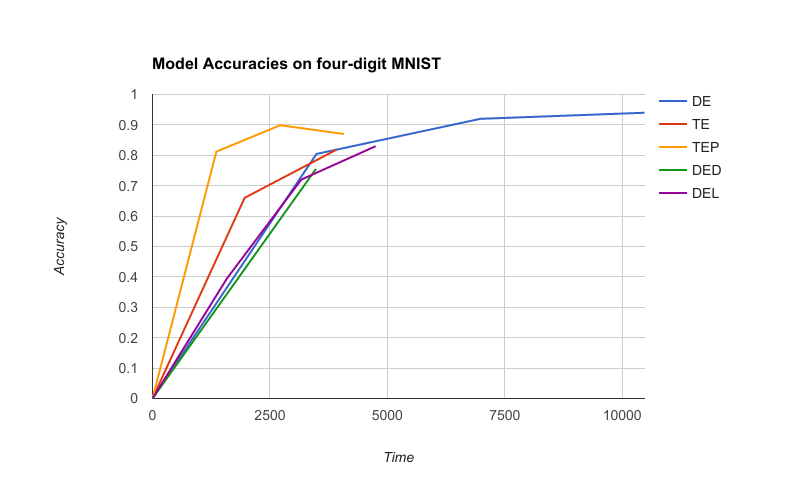
\includegraphics[scale=0.5]{resources/mnist_4_graph.png}
        \caption{Four-digit MNIST without noise.}
        \label{fig:mnist_early_models}
    \end{subfigure}
    \begin{subfigure}[c]{1.0\textwidth}
        \centering
        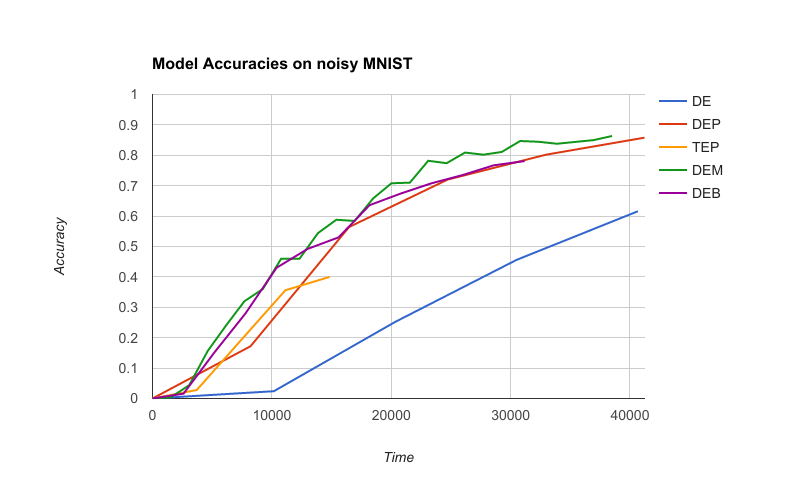
\includegraphics[scale=0.5]{resources/model_experiments.png}
        \caption{Noisy MNIST.}
        \label{fig:mnist_models}
    \end{subfigure}
    \caption{Plot of accuracy vs training time measured in CPU seconds for several models. Each data point comes after one epoch of training.}
\end{figure}


The best variations were evaluated on the more difficult synthetic dataset with random positions and noise. Figure \ref{fig:mnist_models} contains a comparison between some variations of encoder configurations on the noisy MNIST dataset. The three best model configurations (DEM, DEP, DEB) achieved very similar results considering the test accuracy vs training time.



% By training on the simpler four-digit MNIST dataset without noise, we found several viable configurations of encoder and decoder.

% We found various viable models by working on the simpler dataset of four-digit MNIST without noise.




% \subsection{Encoder depth}

\section{Experiments}

Here we discuss comparisons we made between different models.

\subsection{Hardware setup}

The models were implemented in Tensorflow \cite{Tensorflow}, which is a popular open-sourced machine learning framework. The implementation\footnote{\url{https://github.com/HalfLeif/CNN_doc_extraction}} is freely available on Github.

We trained the models on 3 threads on a single Intel(R) Core(TM) i7-4770K @ 3.50GHz. Training a single epoch of Swedish population records took about 28 hours. It would be faster to train using more threads or using GPU acceleration but we were constrained by low access to hardware.




\subsection{Soft vs hard attention}

\subsection{Independent digits} \label{sssec:ind_digits}

\subsection{Multi-year vs single-year loss function}
